\documentclass{exam} % Allows insertion of \question and generally looks nicer

%------------------------------------------------
%	            PACKAGES AND CONFIG
%------------------------------------------------
\usepackage{graphicx} % Required for inserting images
\usepackage{amsmath}
\usepackage{titling}
\usepackage{caption}
\usepackage{amsfonts}
\usepackage{amsthm}
\usepackage{hyperref}
% \usepackage[english]{babel}
\counterwithin*{equation}{section}% Reset equation at \section
\counterwithin*{equation}{subsection}% Reset equation at \subsection
\counterwithin*{equation}{subsubsection}% Reset equation at \subsubsection
\setlength\parindent{0pt}
\hypersetup{
    colorlinks,
    citecolor=black,
    filecolor=black,
    linkcolor=black,
    urlcolor=black
}

%------------------------------------------------
%	                COMMANDS
%------------------------------------------------

\renewcommand\maketitlehooka{\null\mbox{}\vfill}
\renewcommand\maketitlehookd{\vfill\null}
\newcommand{\RomanNumeralCaps}[1]{\MakeUppercase{\romannumeral #1}}
\usepackage[framemethod=TikZ]{mdframed}

\newcounter{prf}[section]\setcounter{prf}{0}
\renewcommand{\theprf}{\arabic{section}.\arabic{prf}}
\newenvironment{prf}[2][]{%
\refstepcounter{prf}%
\ifstrempty{#1}%
{\mdfsetup{%
frametitle={%
\tikz[baseline=(current bounding box.east),outer sep=0pt]
\node[anchor=east,rectangle,fill=red!20]
{\strut Bewijs~\theprf};}}
}%
{\mdfsetup{%
frametitle={%
\tikz[baseline=(current bounding box.east),outer sep=0pt]
\node[anchor=east,rectangle,fill=red!20]
{\strut Bewijs~\theprf:~#1};}}%
}
\mdfsetup{innertopmargin=10pt,linecolor=red!20,%
linewidth=2pt,topline=true,%
frametitleaboveskip=\dimexpr-\ht\strutbox\relax
}
\begin{mdframed}[]\relax%
\label{#2}}{\vspace{0.25cm}\qed\end{mdframed}}
\newcounter{theo}[section]\setcounter{theo}{0}
\renewcommand{\thetheo}{\arabic{section}.\arabic{theo}}
\newenvironment{theo}[2][]{%
\refstepcounter{theo}%
\ifstrempty{#1}%
{\mdfsetup{%
frametitle={%
\tikz[baseline=(current bounding box.east),outer sep=0pt]
\node[anchor=east,rectangle,fill=cyan!20]
{\strut Theorem~\thetheo};}}
}%
{\mdfsetup{%
frametitle={%
\tikz[baseline=(current bounding box.east),outer sep=0pt]
\node[anchor=east,rectangle,fill=cyan!20]
{\strut Theorem~\thetheo:~#1};}}%
}%
\mdfsetup{innertopmargin=10pt,linecolor=cyan!20,%
linewidth=2pt,topline=true,%
frametitleaboveskip=\dimexpr-\ht\strutbox\relax
}
\begin{mdframed}[]\relax%
\label{#2}}{\vspace{0.25cm}\end{mdframed}}
\newcounter{lem}[section]\setcounter{lem}{0}
\renewcommand{\thelem}{\arabic{section}.\arabic{lem}}
\newenvironment{lem}[2][]{%
\refstepcounter{lem}%
\ifstrempty{#1}%
{\mdfsetup{%
frametitle={%
\tikz[baseline=(current bounding box.east),outer sep=0pt]
\node[anchor=east,rectangle,fill=green!20]
{\strut Wet~\thelem};}}
}%
{\mdfsetup{%
frametitle={%
\tikz[baseline=(current bounding box.east),outer sep=0pt]
\node[anchor=east,rectangle,fill=green!20]
{\strut Wet~\thelem:~#1};}}%
}%
\mdfsetup{innertopmargin=10pt,linecolor=green!20,%
linewidth=2pt,topline=true,%
frametitleaboveskip=\dimexpr-\ht\strutbox\relax
}
\begin{mdframed}[]\relax%
\label{#2}}{\vspace{0.25cm}\end{mdframed}}
\newcounter{ex}[section]\setcounter{ex}{0}
\renewcommand{\theex}{\arabic{section}.\arabic{ex}}
\newenvironment{ex}[2][]{%
\refstepcounter{ex}%
\ifstrempty{#1}%
{\mdfsetup{%
frametitle={%
\tikz[baseline=(current bounding box.east),outer sep=0pt]
\node[anchor=east,rectangle,fill=purple!20]
{\strut Voorbeeld~\theex};}}
}%
{\mdfsetup{%
frametitle={%
\tikz[baseline=(current bounding box.east),outer sep=0pt]
\node[anchor=east,rectangle,fill=purple!20]
{\strut Voorbeeld~\theex:~#1};}}%
}%
\mdfsetup{innertopmargin=10pt,linecolor=purple!20,%
linewidth=2pt,topline=true,%
frametitleaboveskip=\dimexpr-\ht\strutbox\relax
}
\begin{mdframed}[]\relax%
\label{#2}}{\vspace{0.25cm}\end{mdframed}}
\newcounter{pro}[section]\setcounter{pro}{0}
\renewcommand{\thepro}{\arabic{section}.\arabic{pro}}
\newenvironment{pro}[2][]{%
\refstepcounter{pro}%
\ifstrempty{#1}%
{\mdfsetup{%
frametitle={%
\tikz[baseline=(current bounding box.east),outer sep=0pt]
\node[anchor=east,rectangle,fill=purple!20]
{\strut Eigenschap~\thepro};}}
}%
{\mdfsetup{%
frametitle={%
\tikz[baseline=(current bounding box.east),outer sep=0pt]
\node[anchor=east,rectangle,fill=purple!20]
{\strut Eigenschap~\thepro:~#1};}}%
}%
\mdfsetup{innertopmargin=10pt,linecolor=purple!20,%
linewidth=2pt,topline=true,%
frametitleaboveskip=\dimexpr-\ht\strutbox\relax
}
\begin{mdframed}[]\relax%
\label{#2}}{\vspace{0.25cm}\end{mdframed}}
\newcounter{app}[section]\setcounter{app}{0}
\renewcommand{\theapp}{\arabic{section}.\arabic{app}}
\newenvironment{app}[2][]{%
\refstepcounter{app}%
\ifstrempty{#1}%
{\mdfsetup{%
frametitle={%
\tikz[baseline=(current bounding box.east),outer sep=0pt]
\node[anchor=east,rectangle,fill=magenta!20]
{\strut Toepassing~\theapp};}}
}%
{\mdfsetup{%
frametitle={%
\tikz[baseline=(current bounding box.east),outer sep=0pt]
\node[anchor=east,rectangle,fill=magenta!20]
{\strut Toepassing~\theapp:~#1};}}%
}
\mdfsetup{innertopmargin=10pt,linecolor=magenta!20,%
linewidth=2pt,topline=true,%
frametitleaboveskip=\dimexpr-\ht\strutbox\relax
}
\begin{mdframed}[]\relax%
\label{#2}}{\vspace{0.25cm}\end{mdframed}}
\newcounter{summ}[section]\setcounter{summ}{0}
\renewcommand{\thesumm}{\arabic{section}.\arabic{summ}}
\newenvironment{summ}[2][]{%
\refstepcounter{summ}%
\ifstrempty{#1}%
{\mdfsetup{%
    frametitle={%
    \tikz[baseline=(current bounding box.east),outer sep=0pt]
    \node[anchor=east,rectangle,fill=violet!20]
    {\strut Samenvatting~\thesumm};}}
}%
{\mdfsetup{%
    frametitle={%
    \tikz[baseline=(current bounding box.east),outer sep=0pt]
    \node[anchor=east,rectangle,fill=violet!20]
    {\strut Samenvatting~\thesumm:~#1};}}%
}
\mdfsetup{innertopmargin=10pt,linecolor=violet!20,%
    linewidth=2pt,topline=true,%
    frametitleaboveskip=\dimexpr-\ht\strutbox\relax
}
\begin{mdframed}[]\relax%
\label{#2}}{\vspace{0.25cm}\end{mdframed}}
\newcounter{vrg}[section]\setcounter{vrg}{0}
\renewcommand{\thevrg}{\arabic{section}.\arabic{vrg}}
\newenvironment{vrg}[2][]{%
\refstepcounter{vrg}%
\ifstrempty{#1}%
{\mdfsetup{%
    frametitle={%
    \tikz[baseline=(current bounding box.east),outer sep=0pt]
    \node[anchor=east,rectangle,fill=teal!20]
    {\strut Vergelijking~\thevrg};}}
}%
{\mdfsetup{%
    frametitle={%
    \tikz[baseline=(current bounding box.east),outer sep=0pt]
    \node[anchor=east,rectangle,fill=teal!20]
    {\strut Vergelijking~\thevrg:~#1};}}%
}
\mdfsetup{innertopmargin=10pt,linecolor=teal!20,%
    linewidth=2pt,topline=true,%
    frametitleaboveskip=\dimexpr-\ht\strutbox\relax
}
\begin{mdframed}[]\relax%
\label{#2}}{\vspace{0.25cm}\end{mdframed}}

\newcommand{\introPage}[1]{

    \vspace*{\fill}
    \begin{center}
        
    \section*{#1}
    \end{center}

    \vspace*{\fill}
}

%------------------------------------------------
%	            START OF DOCUMENT
%------------------------------------------------

\title{Micro}
\author{Pieter Vanderschueren}
\date{Academiejaar 2023-2024}

\begin{document}

\begin{titlingpage}
\maketitle
\end{titlingpage}

\newpage

%------------------------------------------------
%	              INTRODUCTION
%------------------------------------------------

% \introPage{Inleiding}

%------------------------------------------------
%	           TABLE OF CONTENTS
%------------------------------------------------

\newpage

\tableofcontents

\newpage

%------------------------------------------------
%	                INPUTS
%------------------------------------------------

\section{Demand}

\vspace{0.5cm}

\begin{theo}[Demand function]{Demand function and the inverse demand function}
    \begin{itemize}
        \item 
            The demand function $x_D(p)$ illustrates the demand for a certain good at a certain price, see the following illustration:
            \begin{center}
                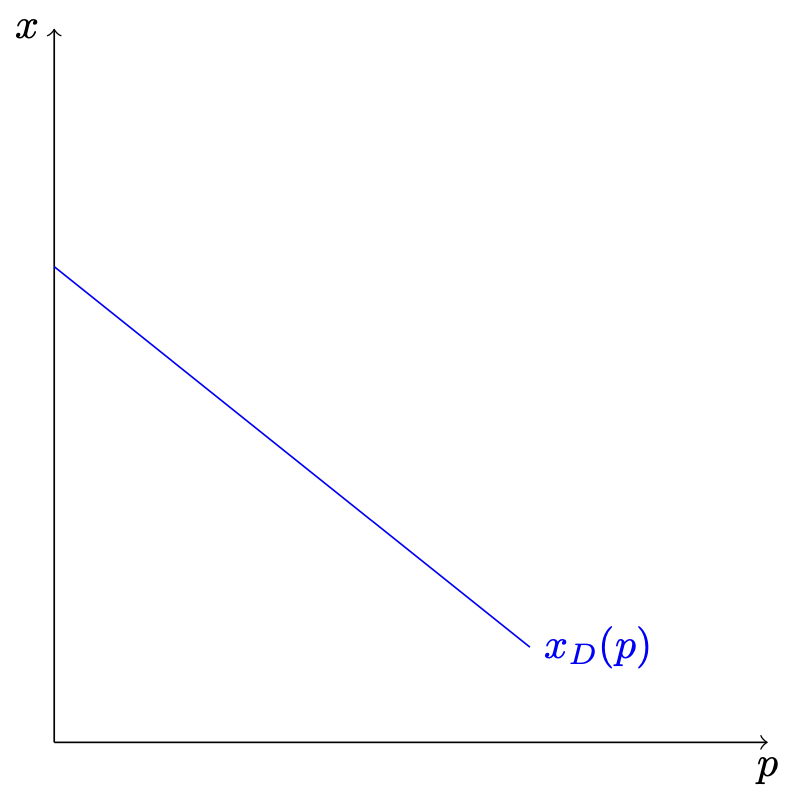
\includegraphics[scale = 0.2]{Images/Demand/DemandFunction.png}
            \end{center}
            The demand function is decreasing: $p \uparrow \ \Rightarrow x_D(p) \downarrow$
        \item  
            The inverse demand function $v(x)$ illustrates the consumers willingness to pay for a good, see the following illustration:
            \begin{center}
                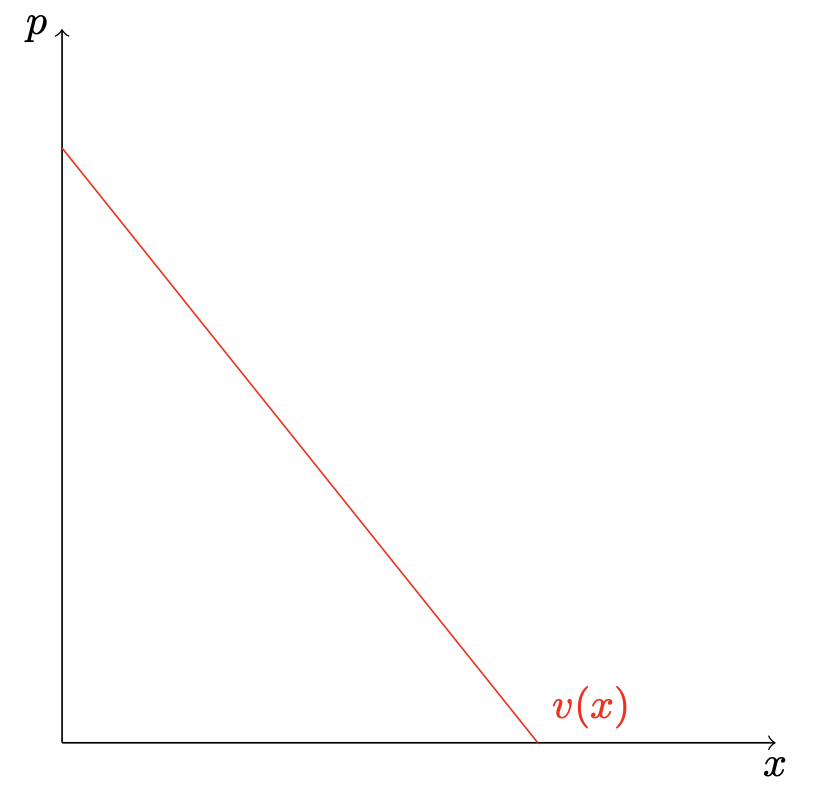
\includegraphics[scale = 0.2]{Images/Demand/InverseDemandFunction.png}
            \end{center}
            An agent will be willing to buy more as long as $v(x) > p$. 
    \end{itemize}
\end{theo}

\newpage

\begin{theo}[Utility function]{Utility function}
    The utility function illustrates the total monetary value of total consumption:
    \begin{equation*}
        u(x) = \int_0^x v(s)ds
    \end{equation*} 
    We can also refer to $v(x)$ as the agent's \textbf{marginal utility function}, since 
    \begin{equation*}
        u'(x) = v(x).
    \end{equation*}
    Since we required $v(x)$ to be decreasing in $x$, this means that $u(x)$ is concave:
    \begin{equation*}
        u''(x) = v'(x) < 0.
    \end{equation*}
    \vspace*{-0.5cm}
\end{theo}

\begin{theo}[Cosumer surplus]{Cosumer surplus}
    The consumer surplus $CS$ is the consumer's utility net of the monetary cost of consumption:
    \begin{equation*}
        CS = u(x) - px = \int_0^x v(s)ds - \int_0^x pds = \int_0^x \left(v(s) - p \right)ds
    \end{equation*}
    Graphically, the consumer surplus is definedned as the area that lies below the inverse demand function, but above the price line:
    \begin{center}
        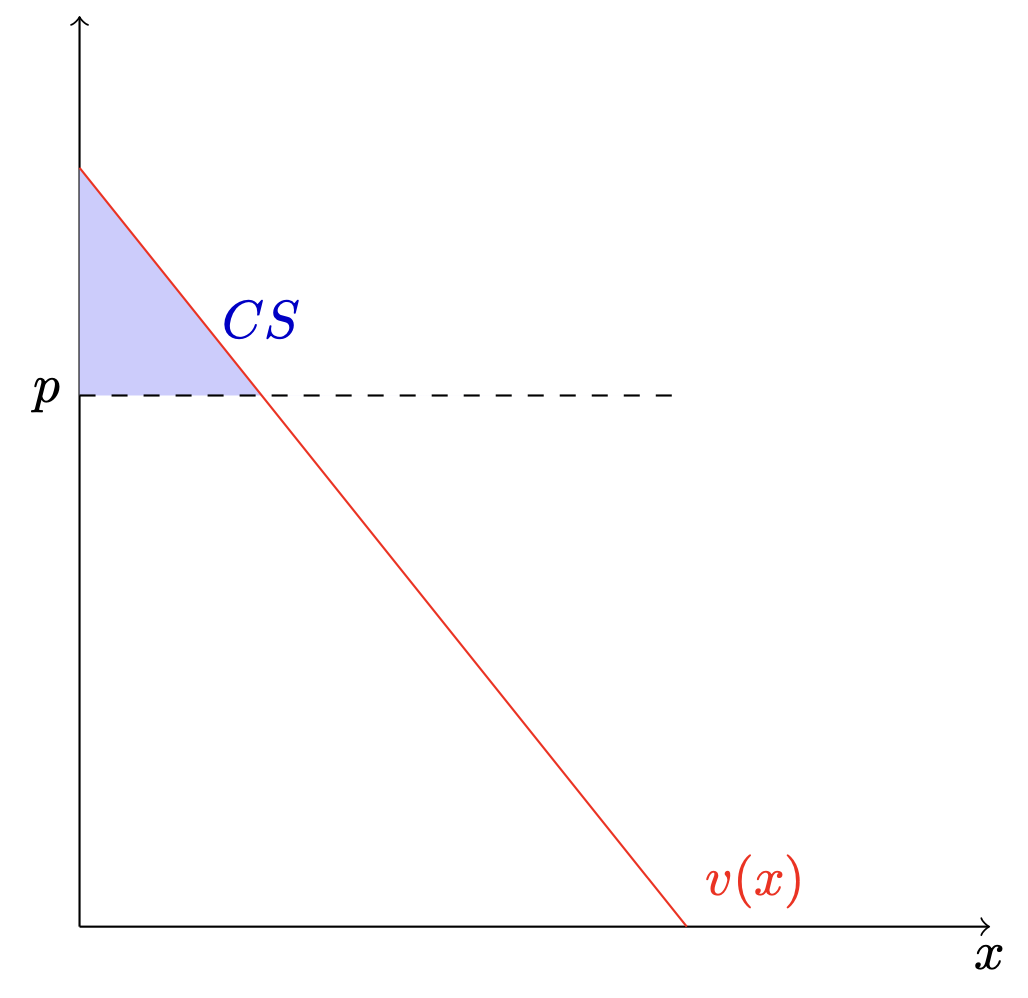
\includegraphics[scale = 0.15]{Images/Demand/ConsumerSurplus.png}
    \end{center}
    When deciding to buy a good, an agent is maximizing consumer surplus, i.e., the net benefit of consumption:
    \begin{equation*}
        \max_x \ CS = \max_x \ u(x) - px
    \end{equation*}
\end{theo}

\end{document}